\documentclass[pdf, autumn, slideColor, nocolorBG]{prosper}
\usepackage{verbatim}
\usepackage{color}
\usepackage{hyperref}
\usepackage{biblatex}
\usepackage{subfig}

%General Short-Cut Commands
\newcommand{\superscript}[1]{\ensuremath{^{\textrm{#1}}}}
\newcommand{\subscript}[1]{\ensuremath{_{\textrm{#1}}}}
\newcommand{\nuc}[2]{\superscript{#2}{#1}}
\newcommand{\FigCaption}[1]{\begin{center}{\tiny{#1}}\end{center}}

%Commands for this document...
\newcommand{\Red}[1]{\textcolor{red}{#1}}


% Bibliography
\bibliography{../library}{}


%Presentation information
\title{Essential Physics Fuel Cycle Modeling \& Analysis}
\subtitle{PhD Defense - September 7\superscript{th}, 2010 - Austin, TX}
\author{Anthony Scopatz}
\email{scopatz@mail.utexas.edu}
\institution{\tiny
Department of Mechanical Engineering, Nuclear Engineering Program\\
The University of Texas at Austin\\
1 University Station, MC R9000, Austin, TX 78712
}

\slideCaption{Scopatz - PhD Defense}

\begin{document}

% make the title slide
\maketitle


% Motivation
\overlays{5}{
\begin{slide}{Motivation}
\FromSlide{1}
\begin{itemize}
    \item Many nuclear fuel cycle simulations are formulated on premade base-case scenarios:

\FromSlide{2}
    \begin{center}
    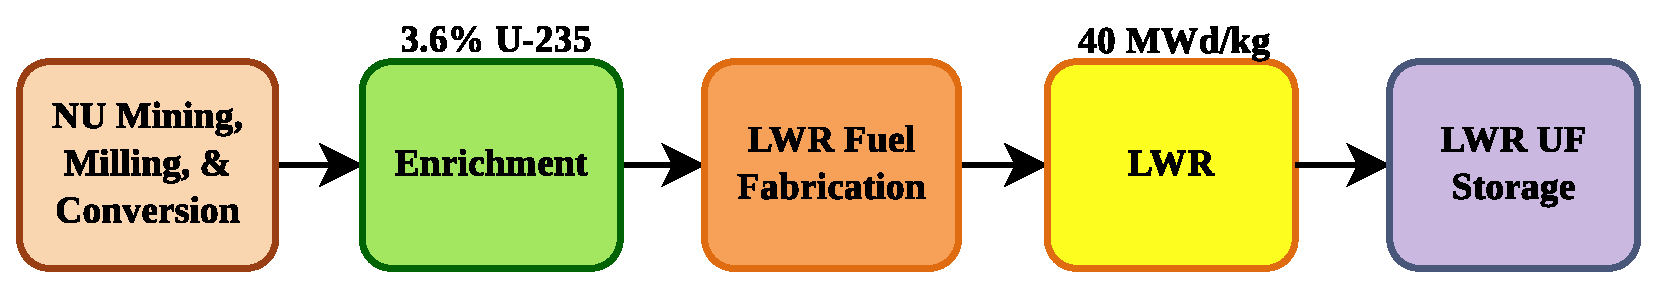
\includegraphics[scale=0.25]{figs/OnceThrough.eps}
    \end{center}

\FromSlide{3}
    \item These base cases are very well studied.

\FromSlide{4}
    \item However, what is \textbf{\textit{not}} well known is 
        how these sample scenarios are affected by perturbations to their 
        initial physical parameters.
            
\FromSlide{1}
\end{itemize}

\FromSlide{5}
\begin{center}
``\textit{Do our parameter choices really give us the `best' solution?}''
\end{center}

\end{slide}}





% Motivation
\begin{slide}{Motivation}
\begin{center}
\begin{figure}
\caption{Physics Modeled versus Execution Time}
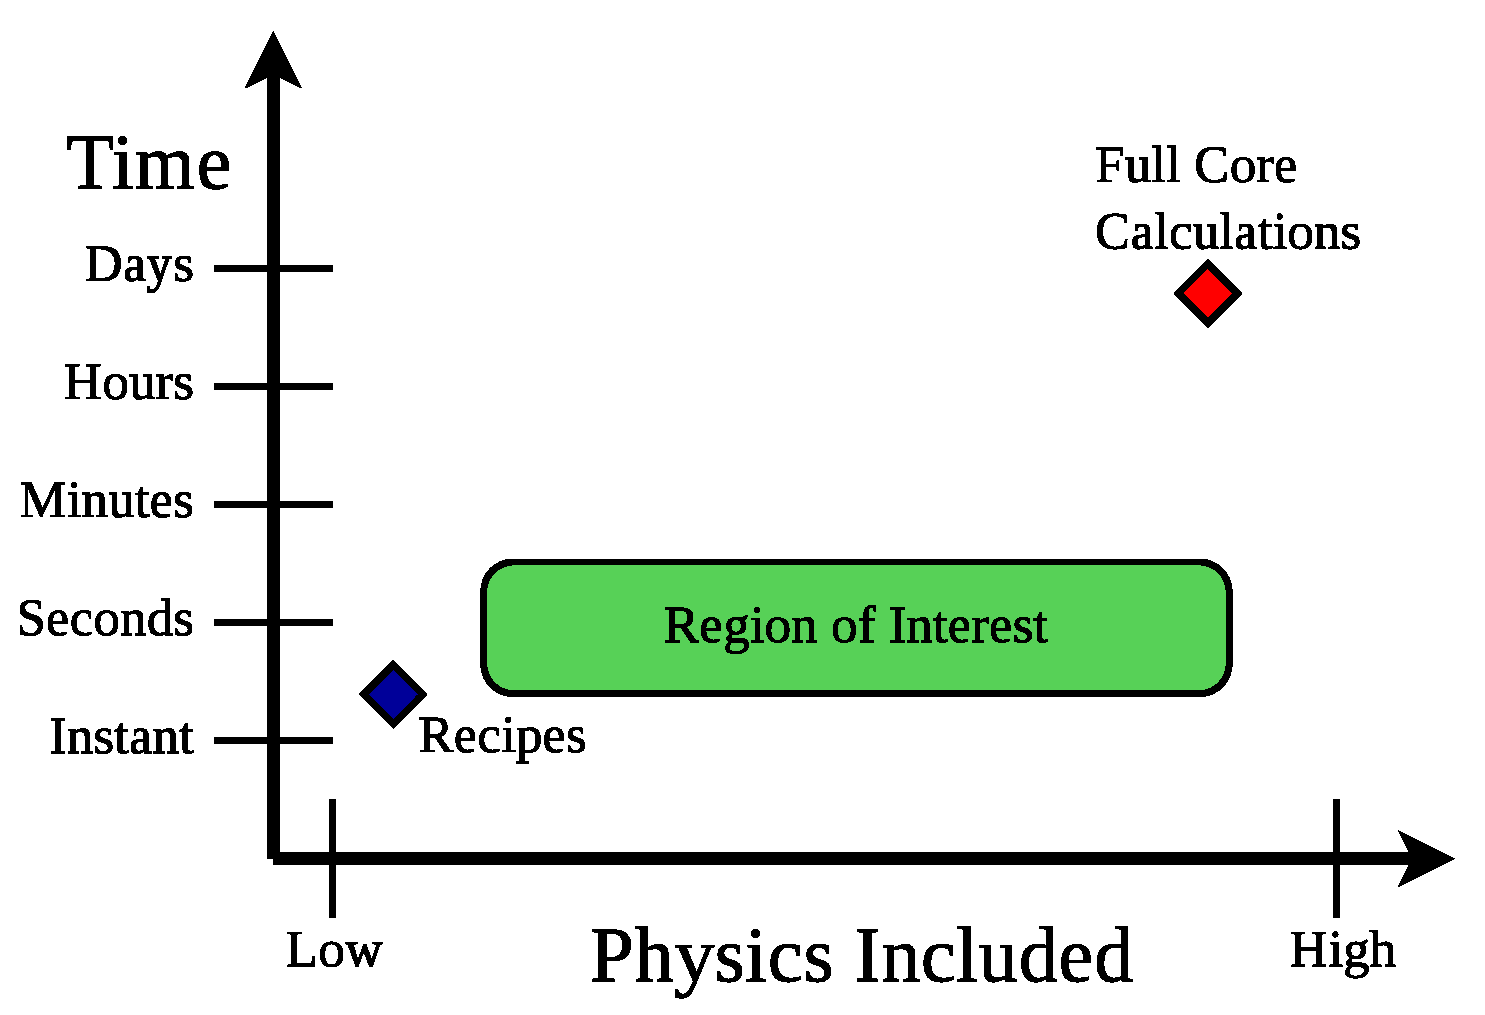
\includegraphics[scale=0.35]{figs/physics_vs_exec_time.eps}
\end{figure}
\end{center}
\end{slide}




% Motivation
\begin{slide}{Motivation}
\small Basic Fuel Cycle Schema:
\begin{center}
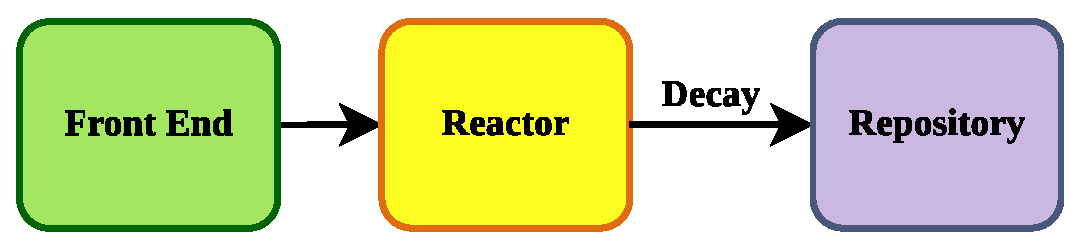
\includegraphics[scale=0.5]{figs/basic_nfc_schema.eps}
\end{center}

Modeling Approaches: \small
\begin{center}
\begin{tabular}{lccc}
\textit{Component}                  & \textit{Recipes}  & \textit{Essential} & \textit{Transport}   \\
\underline{\textbf{Front End:}}     & Recipes           & Physics Models     & Physics Models       \\
\underline{\textbf{Reactor:}}       & Recipes           & Rapid Burnup Code  & Neutron Transport    \\
\underline{\textbf{Repository:}}    & Curve Fits        & Rapid Code         & Neutron Transport    \\
\end{tabular}
\end{center}
\end{slide}





% Motivation
\overlays{2}{
\begin{slide}{Motivation}
\FromSlide{1}
\begin{itemize}
    \item Investigating the region of interest may provide a 
        \textit{transformative} amount of fuel cycle data.  

\FromSlide{2}
    \item However, this requires an entirely new spectrum of tools.

\FromSlide{1}
\end{itemize}


\FromSlide{2}
\setcounter{figure}{1}
\begin{center}
\begin{figure}
\caption{Fuel Cycle Stack}
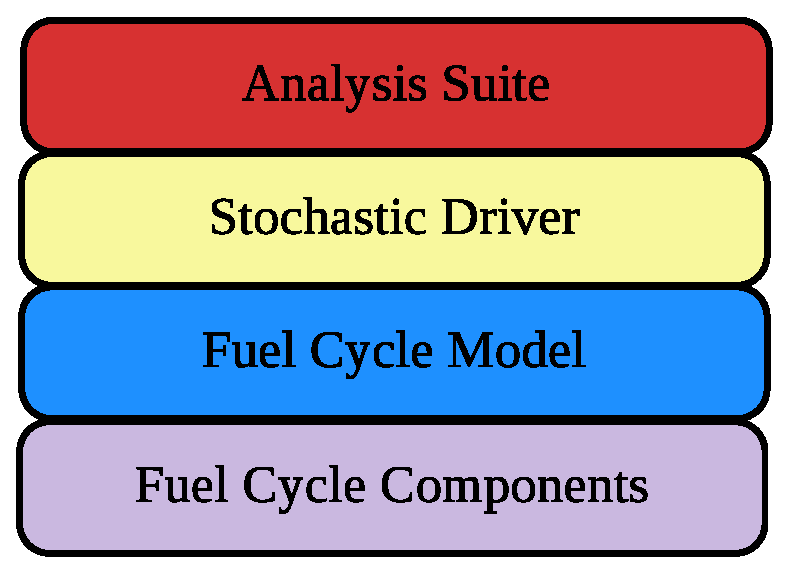
\includegraphics[scale=0.35]{figs/fc_stack.eps}
\end{figure}
\end{center}

\end{slide}}



% Definition
\begin{slide}{Definition}
\vspace{3.0cm}
\begin{center}
\textit{Essential physics} models remain physically valid under perturbations
in the locality of the region that they are defined and do not compute
extraneous parameters.  
\end{center}
\end{slide}




% A Path Forward
\overlays{4}{
\begin{slide}{A Path Forward}
\FromSlide{1}
\begin{itemize}
    \item Develop a set of fuel cycle component models which 
        preserve basic physics (largely focused on a one-enegy 
        group reactor model, R1G).

\FromSlide{2}
    \item Investigate a categorical set of fuels cycles using
        the above components. (These are largely linear 
        perturbations of previous base-case studies.)

\FromSlide{3}
    \item Extend the fuel cycle model to perturb continuous 
        variables.  This requires a stochastic driving mechanism
        to run.  Moreover, it requires entropy-based measures to
        analyze.

\FromSlide{4}
    \item Model the reactor compoent with 
        multiple energy groups (RMG).  This enables the study 
        of reactors and fuel cycles forbidden in the R1G regime.

\FromSlide{1}
\end{itemize}
\end{slide}}




% R1G
\begin{slide}{R1G}
\vspace{3.5cm}
\begin{center}
\Large
One-Group Reactor Model
\end{center}
\end{slide}





% R1G
\begin{slide}{R1G}
\begin{center}
\begin{figure}
\caption{Reactor Model [1]}
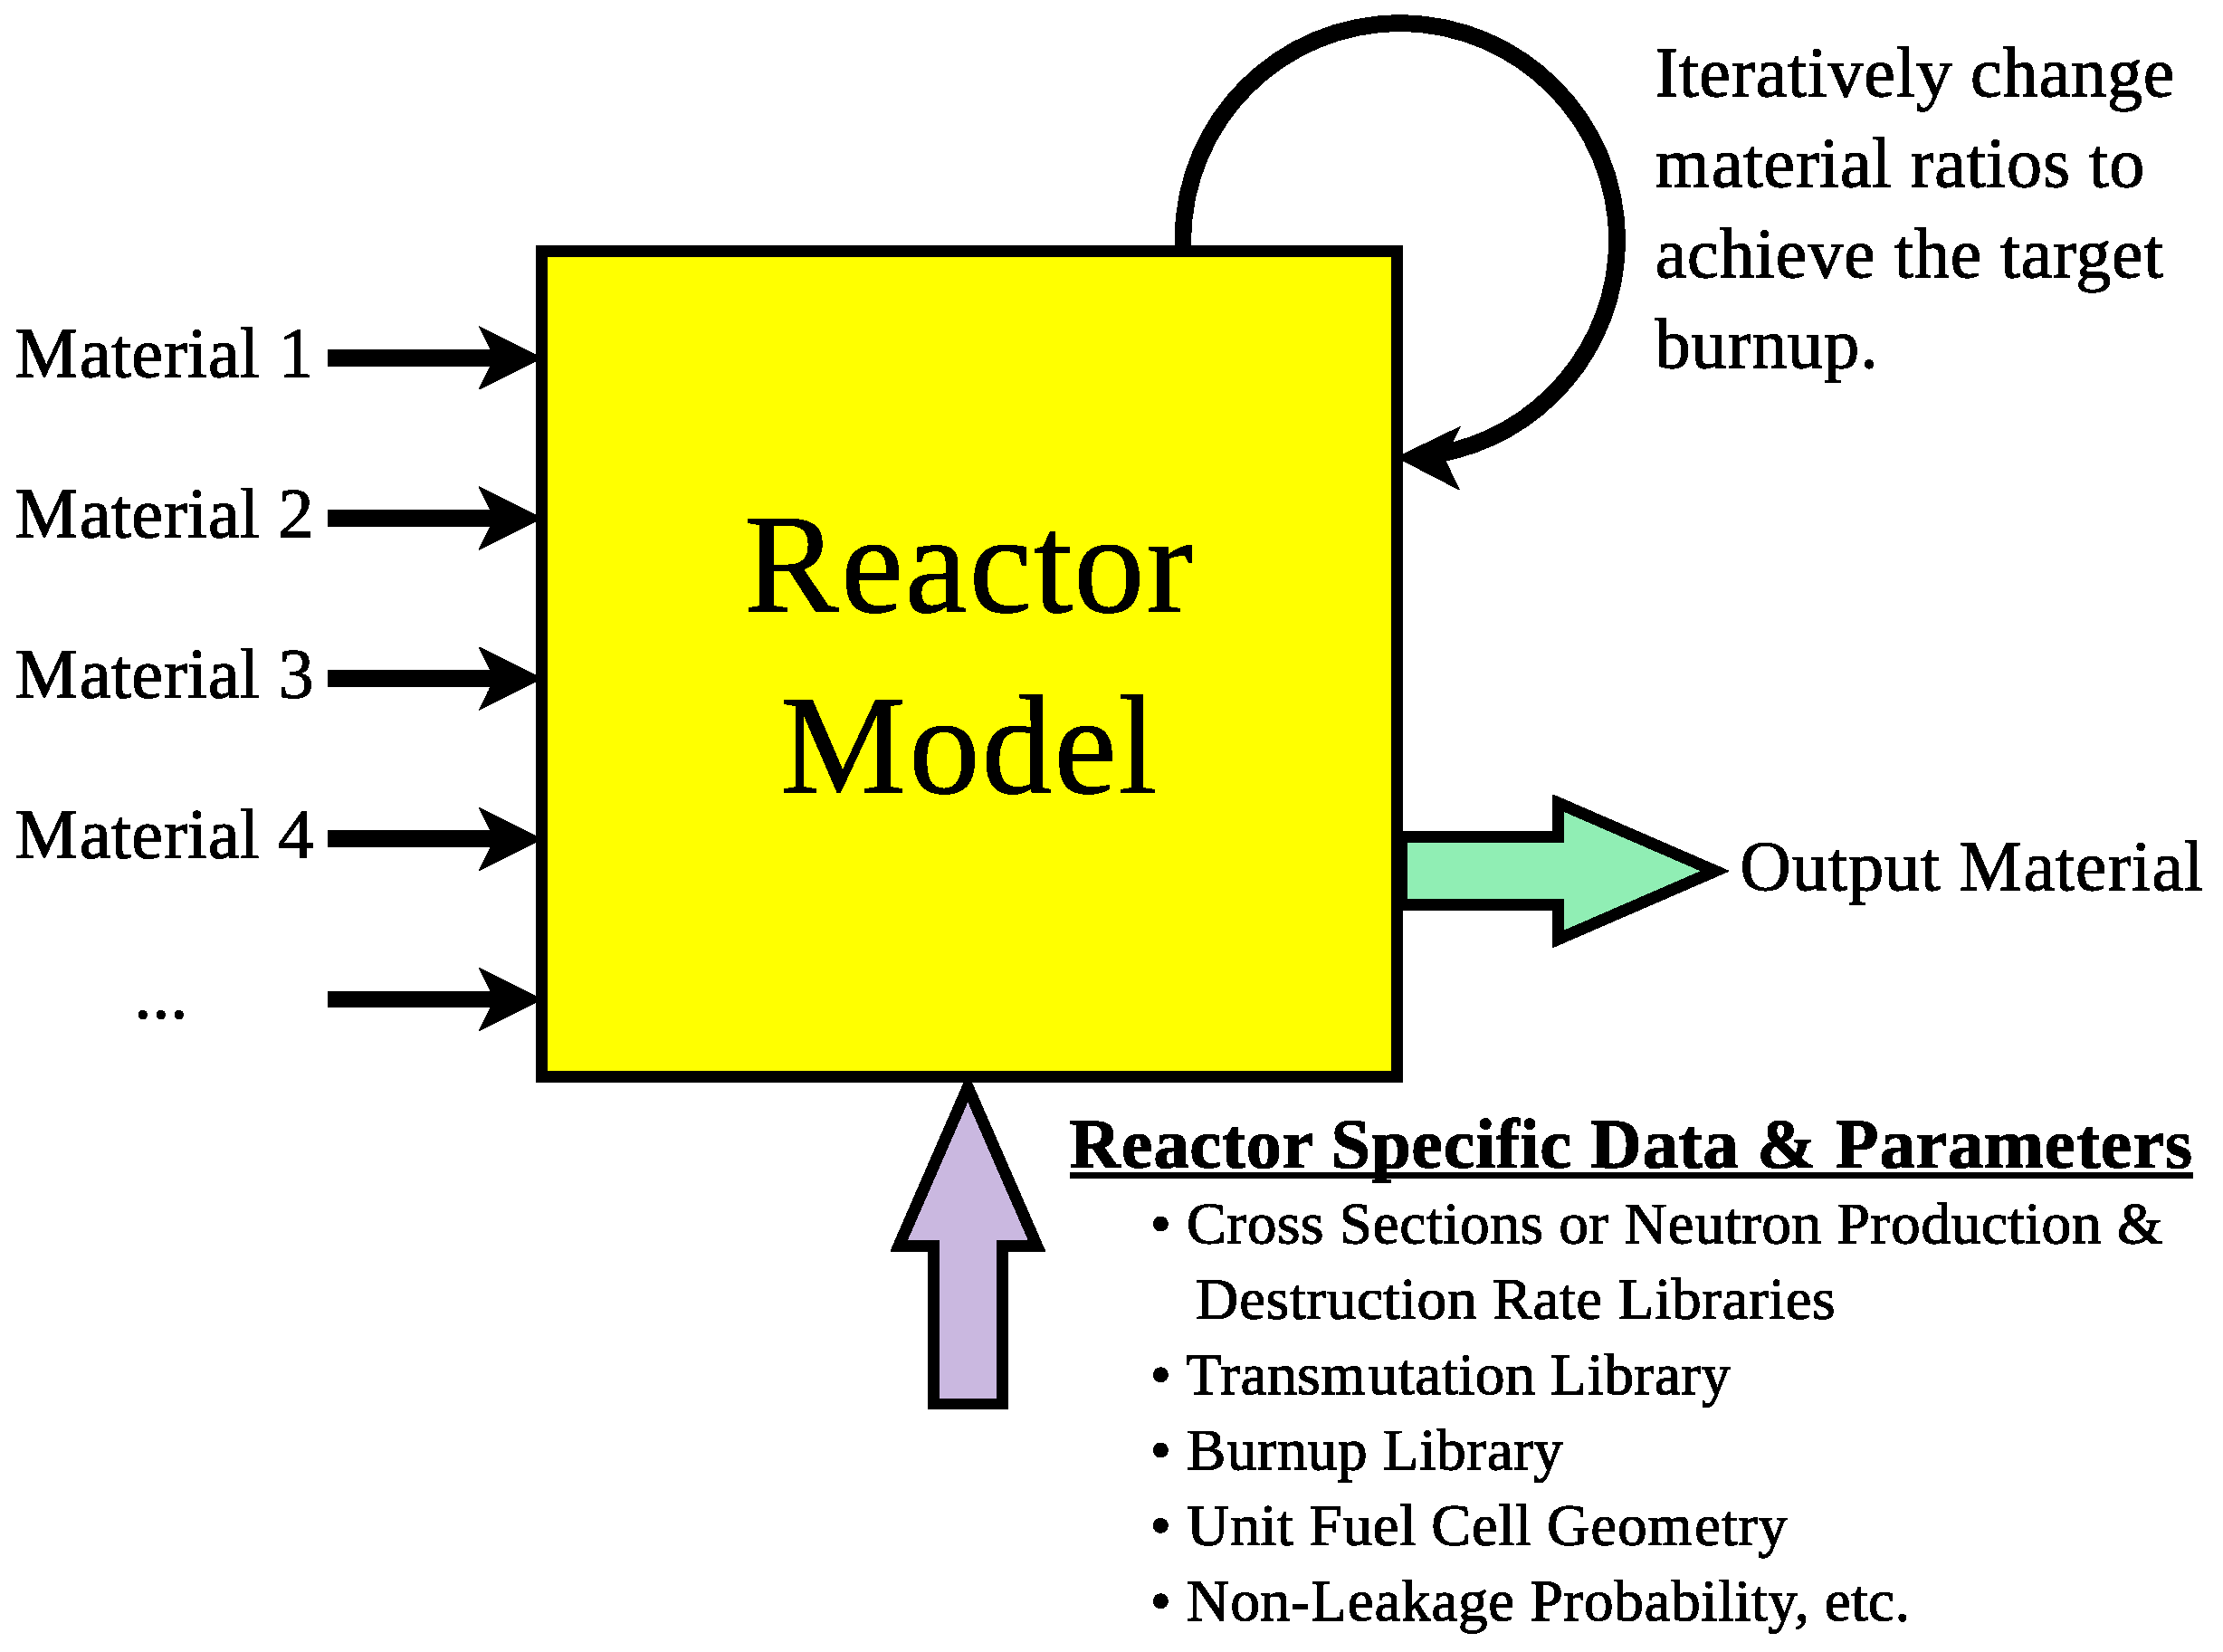
\includegraphics[scale=0.20]{figs/reactor_model.eps}
\end{figure}
\end{center}
\end{slide}



% R1G Notation
\begin{slide}{R1G Notation}
\vspace{0.75cm}
\begin{center}
\begin{table}
\caption{One-Group Reactor Symbols}
\tiny
\begin{tabular}{|l|c|c|}
\hline
\textbf{Name} & \textbf{Symbol} & \textbf{Units} \\
\hline
Fluence & $F = \int_0^t \phi dt^\prime = \phi \int_0^t dt^\prime = \phi \times t \cdot \frac{24 \cdot 3600 \cdot 10^3}{10^{24}}$ & [n/kb] \\
Nuclide Subscript & $i$ (or $j$) & [1/kg\subscript{$i$}] \\
Region Superscript & $Q$ & [unitless] \\
Mass Weights & $m_i^Q = \frac{N_i^Q}{N_{\mbox{IHM}}} = \frac{n_i^Q A_i}{A_{\mbox{IHM}}} \cdot \frac{\rho^Q\cdot\mbox{MW}^F}{\rho^F\cdot\mbox{MW}^Q} \frac{V^Q}{V^F}$ & [kg$_i^Q$/kgIHM] \\
Burnup & $\mbox{BU}(F) = \sum_i m_i^F \cdot \mbox{BU}_i(F)$ & [MWd/kgIHM] \\
Prod \& Des Rates & $p_i(F), d_i(F)$ & [n/s/flux/kg$_i$]\\ 
Transmutation Matrix & $T_{ij}(F)$ & [kg$_j$/kg$_i$] \\
Multiplication Factor & $k(F) = \frac{P(F)}{D(F)}$ & [unitless] \\
\hline
\end{tabular}
\end{table}
\end{center}
\end{slide}





% R1G
\overlays{2}{
\begin{slide}{R1G}
\FromSlide{1}
\begin{center}
Starting with ORIGEN generated fluence-dependent, nuclide specific data, we know:

\setcounter{figure}{3}
\begin{figure}
\subfloat[prod \& des rates,]{\includegraphics[scale=0.21]{../one_group_method/figs/Fig02.eps}}
\subfloat[burnups,]{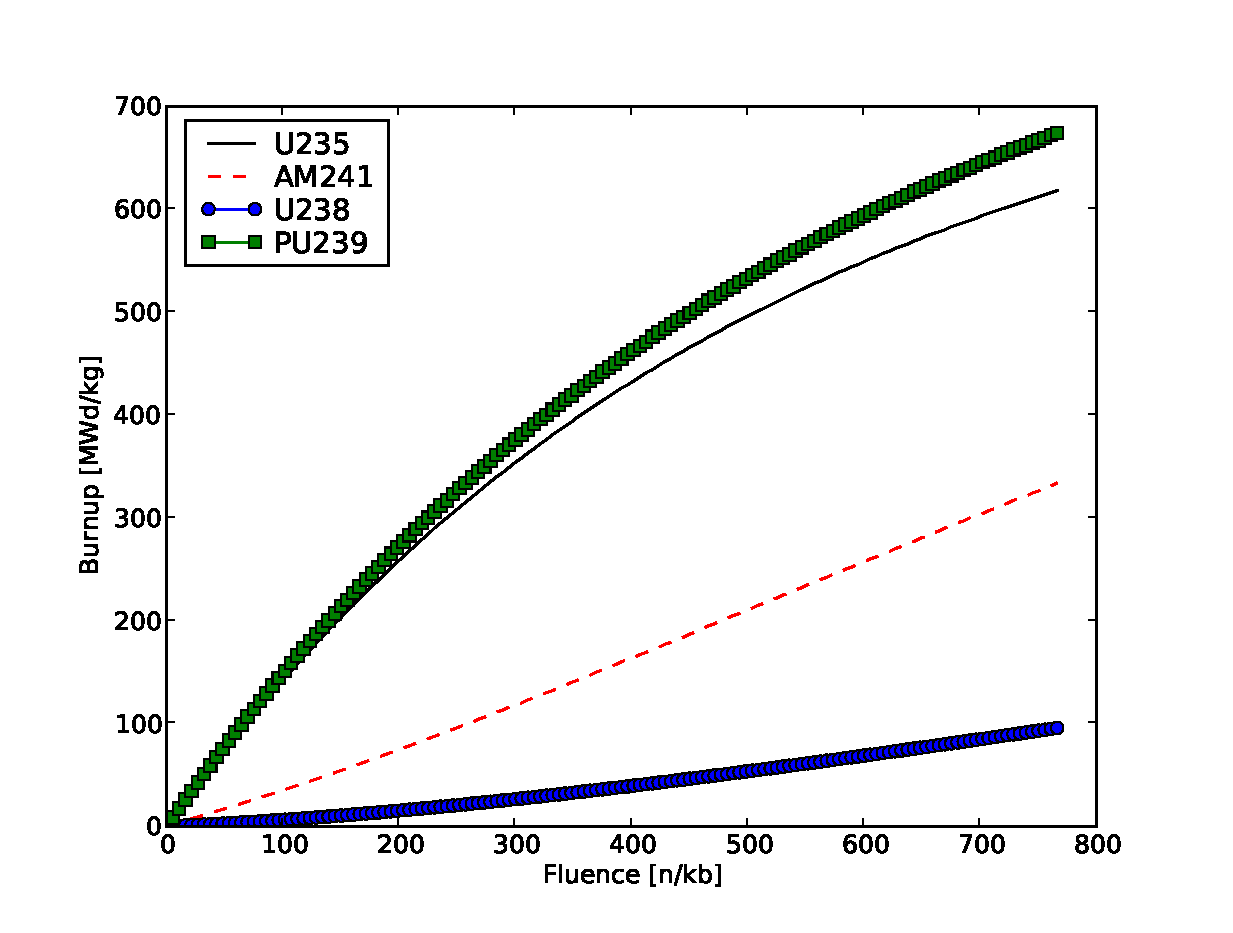
\includegraphics[scale=0.21]{../one_group_method/figs/Fig03.eps}}
\subfloat[transmutation matrices.]{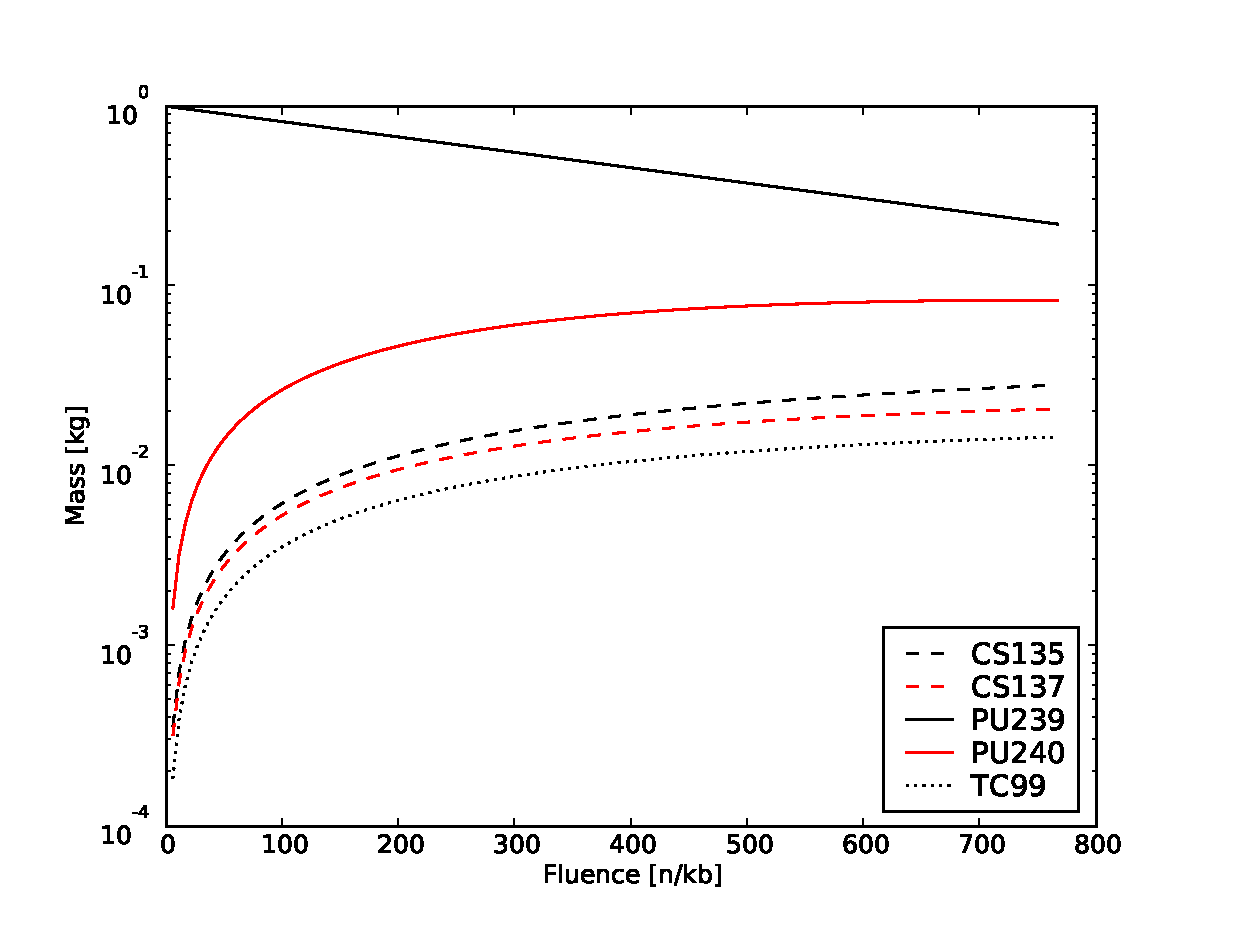
\includegraphics[scale=0.21]{../one_group_method/figs/Fig01.eps}}
\caption{Reactor Data Library (for FR \nuc{Pu}{239})}
\end{figure}

\end{center}

\FromSlide{2}
\footnotesize
To obtan a specific reactor, the above data must be folded together.
\end{slide}}



% R1G Library Collapse
\overlays{4}{
\begin{slide}{R1G Library Collapse}
\FromSlide{1}
\begin{itemize}
    \item We now need to collapse our general library down to a specific reactor at hand.

\FromSlide{2}
    \item Using a two-region fuel pin cell model, denote the mass weight of each initial 
        isotope $i$ in the fuel as $m^F_i$ and the in the coolant as $m^C_i$.

\FromSlide{3}
    \item Then, a mass-weighted linear combination of all of the library
        parameters computes the full-core values.

\FromSlide{4}
    \item For example, 

        \[ P(F) = P_{NL} \cdot p^F(F) = P_{NL} \sum^I_i m^F_i \cdot p^F_i(F) \]
\FromSlide{1}
\end{itemize}
\end{slide}}





% R1G
\begin{slide}{R1G}
\begin{center}
\begin{figure}
\caption{Linearly Weighted Fast Reactor Data}
\subfloat[Burnup]{\includegraphics[scale=0.31]{../one_group_method/figs/Fig05.eps}}
\subfloat[Multiplication Factor]{\includegraphics[scale=0.31]{../one_group_method/figs/Fig06.eps}}
\end{figure}
\end{center}
\end{slide}




% R1G 
\overlays{3}{
\begin{slide}{R1G}
\FromSlide{1}
\begin{minipage}[t]{0.49\textwidth}
\setcounter{figure}{5}
\begin{center}
\begin{figure}
\caption{Fast Reactor\\ Discharge Composition}
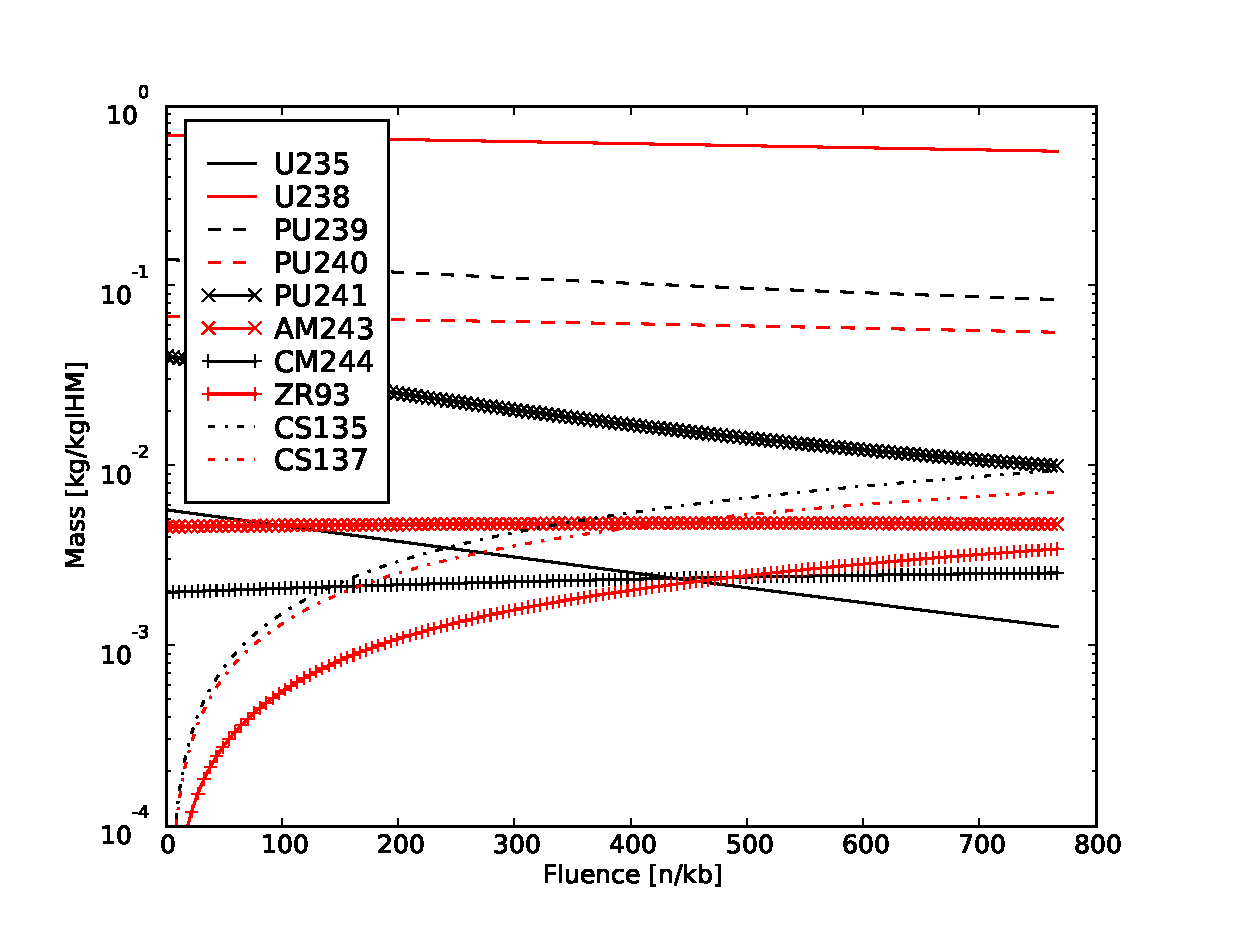
\includegraphics[scale=0.3]{../one_group_method/figs/Fig07.eps}
\end{figure}
\end{center}
\end{minipage}
\begin{minipage}[t]{0.49\textwidth}
\small
\begin{itemize}
    \item The transmutation matrices may be similarly weighted by inital composition.

\FromSlide{2}
    \item From the criticality calculation above we also know the discharge fluence, Fd [n/kb].

\FromSlide{3}
    \item Therefore the used fuel composition is known by taking the nuclide mass weights at 
            Fd in Figure 6.

\FromSlide{1}
\end{itemize}
\end{minipage}
\end{slide}}




% R1G Benchmark
\begin{slide}{R1G Benchmark}
\tiny
\begin{table}[htbp]
\begin{center}
\caption{LWR Benchmark to OECD Burnup Credit [2]}
\begin{tabular}{|l|c|c|c|c|}
\hline
\textbf{Nuclide} & \textbf{OECD [2] [w/o]} & \textbf{$\sigma$ of OECD [\%]} & \textbf{Results [w/o]} & \textbf{\% Difference} \\
\hline
\nuc{U}{234}     & 0.0178  & 9.0  & 0.0184  & +3.6  \\
\nuc{U}{235}     & 0.8001  & 8.1  & 0.7079  & -11.5 \\
\nuc{U}{236}     & 0.4840  & 2.6  & 0.4781  & -1.2  \\
\nuc{U}{238}     & 93.3333 & 0.2  & 93.6109 & +0.3  \\
\nuc{Np}{237}    & 0.0614  & 9.4  & 0.0584  & -5.0  \\
\nuc{Pu}{238}    & 0.0226  & 13.9 & 0.0185  & -18.1 \\
\nuc{Pu}{239}    & 0.5991  & 7.1  & 0.5104  & +14.8 \\
\nuc{Pu}{240}    & 0.2389  & 5.3  & 0.2591  & +8.5  \\
\nuc{Pu}{241}    & 0.1636  & 6.9  & 0.1445  & -11.7 \\
\nuc{Pu}{242}    & 0.0602  & 8.4  & 0.0563  & -6.5  \\
\nuc{Am}{241}    & 0.0047  & 5.3  & 0.0032  & -30.8 \\
\nuc{Am}{243}    & 0.0148  & 10.4 & 0.0116  & -21.3 \\
\hline
\end{tabular}
\end{center}
\end{table}
\end{slide}



% R1G Bechmark Notes
\overlays{2}{
\begin{slide}{R1G Bechmark Notes}
\FromSlide{1}
\begin{itemize}
    \item This benchmark compares an OECD study for a 40 MWd/kgIHM burn with no cooling.

    \item This result shows the R1G matches the burnup credit to within two standard 
        deviations for most actinides.

\FromSlide{2}
    \item \nuc{Am}{241} is the only nuclide showing a relatively higher departure.

    \item This sepcies is formed through \nuc{Pu}{241} decay.

    \item \nuc{Am}{241} would thus match better if a constant flux or 
        if zero reloading times were not assumed.

\FromSlide{1}
\end{itemize}
\end{slide}}




% R1G Fuel Cycle Example: RU
\overlays{3}{
\begin{slide}{R1G Fuel Cycle Example: RU}
\FromSlide{1}
\begin{minipage}[t]{0.49\textwidth}
\small
\begin{itemize}
    \item Recyclable Uranium (RU) is obtained by reprocessing used fuel.

\FromSlide{2}
    \item The RU fuel cycle was split into three energy-equivelent bases which 
        were then compared.

\FromSlide{3}
    \item All options share a common front \& back end fuel cycle.  Therefore
        cost-benefit analyses focus on the differening components.

\FromSlide{1}
\end{itemize}
\end{minipage}
\begin{minipage}[t]{0.49\textwidth}
\setcounter{figure}{6}
\begin{center}
\begin{figure}
\caption{RU Fuel Cycles}
\includegraphics[scale=0.25]{../one_group_method/figs/Fig08.eps}
\end{figure}
\end{center}
\end{minipage}
\end{slide}}





% R1G Fuel Cycle Example: RU
\overlays{4}{
\begin{slide}{R1G Fuel Cycle Example: RU}
\FromSlide{1}
\begin{minipage}[t]{0.49\textwidth}

\setcounter{figure}{7}
\begin{center}
\begin{figure}
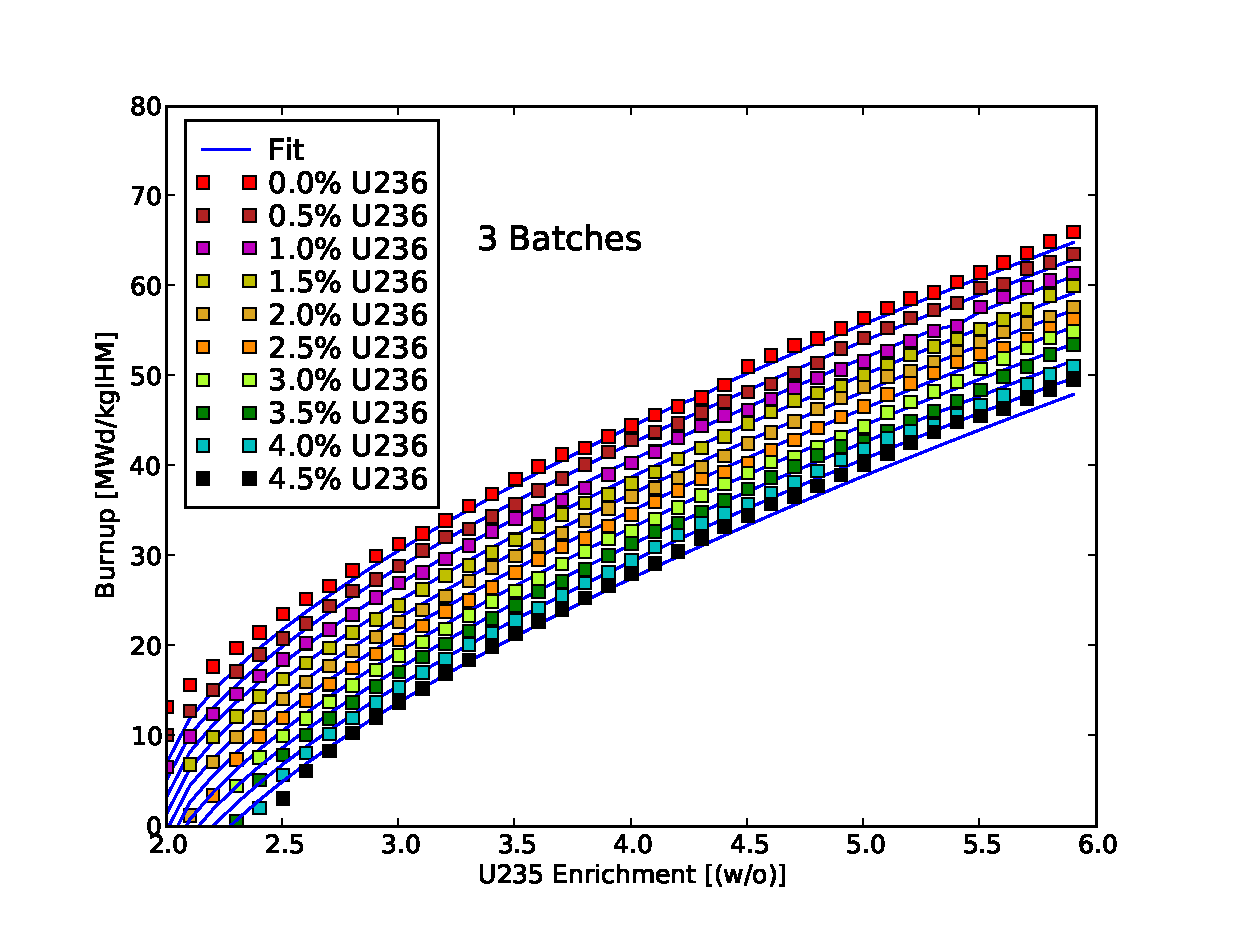
\includegraphics[scale=0.32]{../one_group_method/figs/Fig14.eps}
\caption{Burnup Model Fit for LWRs}
\end{figure}
\end{center}

\end{minipage}
\begin{minipage}[t]{0.49\textwidth}
\footnotesize
\begin{itemize}
    \item RU utility may be further parameterized as a function of \nuc{U}{235},
        \nuc{U}{236}, and the batch loading scheme.  (Not possible for FRs.)

\FromSlide{2}
    \item In Figure 8, data points were calculated and blue lines represent 
        a best-fit curve.

\FromSlide{3}
    \item The 0\% \nuc{U}{236} curve represents a standard LWR.

\FromSlide{4}
    \item This further reduces the computational load of the R1G while remaining 
        perturbable.

\FromSlide{1}
\end{itemize}
\end{minipage}
\end{slide}}





% R1G Fuel Cycle Example: RU
\begin{slide}{R1G Fuel Cycle Example: RU}
\begin{center}
\begin{figure}
\caption{RU Blend Cycle with Mass Balances}
\includegraphics[scale=0.35]{../one_group_method/figs/Fig17.eps}
\end{figure}
\end{center}
\end{slide}





%
% OMG next section
%

% Fuel Cycle Sensitivity Study
\begin{slide}{Sensitivity Study}
\vspace{3.5cm}
\begin{center}
\Large
Fuel Cycle Sensitivity Study
\end{center}
\end{slide}





% Sensitivity Methodology Overview
\overlays{4}{
\begin{slide}{Sensitivity Methodology Overview}
\FromSlide{1}
\begin{itemize}
    \item Here, the system-wide impact of physical parameter perturbations is quantified.

\vspace{0.5cm}
\FromSlide{2}
    \item This is done by looking for linear, 1D sensitivity coefficients for each parameter
        to the \underline{repository capacity} response, measured in [PWh].   

\vspace{0.5cm}
\FromSlide{3}
    \item Denote these sensitivity coefficients as $S_x$ for a small change in an input parameter $x$.

\vspace{0.5cm}
\FromSlide{4}
    \item Sensitivity coefficients are presented for 10\% 
        changes in $x$ from assumed base-case values.

\FromSlide{1}
\end{itemize}
\end{slide}}







% Sensitivity Methodology Overview
\overlays{5}{
\begin{slide}{Sensitivity Methodology Overview}
\FromSlide{1}
\begin{itemize}
\FromSlide{1}
    \item The basic algorithm is as follows:

\tiny
\FromSlide{2}
        \begin{enumerate}
            \item For each input parameter $x$, change its base-case value $x_0$ by $\pm10\%$.
                \[ x \to (1 \pm 0.1)x_0 \]

            \FromSlide{3}
            \item If $x$ is a separation efficiency (SE), instead perturb by $\pm$ ``one nine''
                worth of separations.
                \[ x = 0.999 \to x \in \{0.99, 0.9999\} \]

            \FromSlide{4}
            \item Meanwhile, maintain all other parameters ($y, z, \ldots$) at their
                base-case values.
                \[ y, z, \ldots \to y_0, z_0, \ldots \]    

            \FromSlide{5}
            \item Calculate the new repository capacity response, $R$, by the perturbed cycle and record 
                the sensitivity as the percent change from the base-case response, $R_0$.
                \[ S_{\pm x} = \left(\frac{R}{R_0} - 1\right) \times 100 \]

        \FromSlide{2}
        \end{enumerate}

\FromSlide{1}
\end{itemize}
\end{slide}}



% Fuel Cycle
\overlays{2}{
\begin{slide}{Fuel Cycle}
\FromSlide{1}
\begin{itemize}
    \item The essential physics models from before were
        used it to study a Fast Reactor (FR), Light
        Water Reactor (LWR) symbiotic scenario 
        analogous to Scheme 3a of a 2006 OECD report [3].
\end{itemize}

\FromSlide{2}
\setcounter{figure}{9}
\begin{center}
\begin{figure}
\includegraphics[scale=0.2]{../one_group_method/figs/Fig09.eps}
\caption{LWR-FR Fuel Cycle}
\end{figure}
\end{center}
\end{slide}}




% Fuel Cycle
\overlays{3}{
\begin{slide}{Fuel Cycle}
\FromSlide{1}
\small
With perturbable components, over 30 independent physical 
parameters may be adjusted in the fuel cycle.
\FromSlide{2}
\setcounter{figure}{10}
\begin{figure}
\begin{center}
\includegraphics[scale=0.2]{figs/LWR_FR_FC_knobs.eps}
\caption{LWR-FR Cycle with Parameters}
\end{center}
\end{figure}
\FromSlide{3}
\small
Sensitivity results are computed from equilibrium values derived from 
a full treatment of the preceeding, transient cycles.
\end{slide}}




% Base Case Parameter Definition
\begin{slide}{Base Case Parameter Definition}
\tiny
\begin{center}
\begin{tabular}{|l||c|c|}
\hline
\textbf{Input Parameter $x$} & \textbf{Value} & \textbf{Units} \\
\hline
LWR Burnup & 50.0 & MWd/kgIHM \\
\hline
LWR Fuel to Moderator Ratio & 0.301 & \\
\hline
LWR UF Storage Time & 60 & years \\
\hline
SE of U from LWR UF & 0.999 & \\
\hline
SE of NP from LWR UF & 0.999 & \\
\hline
SE of PU from LWR UF & 0.999 & \\
\hline
SE of AM from LWR UF & 0.999 & \\
\hline
SE of CM from LWR UF & 0.999 & \\
\hline
SE of CS from LWR UF & 0.999 & \\
\hline
SE of SR from LWR UF & 0.999 & \\
\hline
FR Burnup & 140.0 & MWd/kgIHM \\
\hline
FR TRU Conversion Ratio & 0.50 & \\
\hline
Max Fraction of Lanthanide in FR Fuel & 0.0005 & Atoms/TRU Atom \\
\hline
FR UF Storage Time & 3 & years \\
\hline
Storage Before Disposal & 50 & years \\
\hline
\end{tabular}
\end{center}
\end{slide}



% Base Case Parameter Definition
\begin{slide}{Base Case Parameter Definition}
\tiny
\begin{center}
\begin{tabular}{|l||c|c|}
\hline
\textbf{Input Parameter $x$} & \textbf{Value} & \textbf{Units} \\
\hline
SE of U from FR UF & 0.999 & \\
\hline
SE of NP from FR UF & 0.999 & \\
\hline
SE of PU from FR UF & 0.999 & \\
\hline
SE of AM from FR UF & 0.999 & \\
\hline
SE of CM from FR UF & 0.999 & \\
\hline
SE of CS from FR UF & 0.999 & \\
\hline
SE of SR from FR UF & 0.999 & \\
\hline
Density of Host Rock & 2580 & kg/m\superscript{3} \\
\hline
Specific Heat of Host Rock & 840 & J/kg-K \\
\hline
Thermal Conductivity of Host Rock & 1.626 & W/m-K \\
\hline
Heat Loss Factor During Ventilation  & 0.7 & \\
\hline
Drift diameter & 5.5 & m \\
\hline
Ventilation System On Time & 50 & years \\
\hline
Ambient Environment Temperature & 20 & C \\
\hline
Distance Between Drifts & 81 & m \\
\hline
\end{tabular}
\end{center}
\end{slide}






% Fuel Cycle Benchmark
\begin{slide}{Fuel Cycle Base Case Benchmark}
\tiny
\begin{center}
\begin{tabular}{|l||c||c|c||c|c|}
\hline
\textbf{Scheme 3a}     & \textbf{NEA [3]} & \textbf{Model\superscript{1}} & \textbf{\% Diff} & \textbf{Model\superscript{2}} & \textbf{\% Diff} \\
\hline
Electricity Share: LWR & 0.632       & 0.619459             & -2.0244 & 0.634907             & +0.4579 \\
\hline
Electricity Share: FR  & 0.368       & 0.380541             & +3.2955 & 0.365093             & -0.7962 \\
\hline
FR UF: U               & 0.698       & 0.713806             & +2.2143 & 0.715224             & +2.4082 \\
\hline
FR UF: NP              & 0.0065      & 0.00661961           & +1.8070 & 0.00685174           & +5.1335 \\
\hline
FR UF: PU              & 0.266       & 0.248059             & -7.2327 & 0.248319             & -7.1204 \\
\hline
FR UF: AM              & 0.02        & 0.0226796            & 11.8152 & 0.0217317            & +7.9687 \\
\hline
FR UF: CM              & 0.0098      & 0.00883517           & -10.920 & 0.00787319           & -24.4730\\
\hline
HLW: U                 & 0.013324    & 0.0132681            & -0.4213 & 0.0134448            & +0.8984 \\
\hline
HLW: NP                & 2.26542E-05 & 2.4079E-05           & +5.9173 & 2.41083E-05          & +6.0316 \\
\hline
HLW: PU                & 0.000704797 & 0.000658893          & -6.9668 & 0.000632361          & -11.4548\\
\hline
HLW: AM                & 5.03426E-05 & 5.63068E-05          & 10.5923 & 5.12344E-05          & +1.7405 \\
\hline
HLW: CM                & 2.18151E-05 & 1.99031E-05          & -9.6068 & 1.67094E-05          & -30.5563\\
\hline
HLW: FP                & 0.985876    & 0.985973             & +0.0098 & 0.985831             & -0.0046 \\
\hline
\end{tabular}
\end{center}

1: Model with initial LWR \nuc{U}{235} enrichment of 4.2 w/o. 

2: Model with LWR discharge burnup of 50 MWd/kg.
\end{slide}




% Fuel Cycle Dynamics
\begin{slide}{Fuel Cycle Dynamics}
\begin{center}
\begin{figure}
\caption{Input Streams to FR [kg/kgIHM]}
\includegraphics[scale=0.4]{../se_sensitivity/figs/MassStreams.eps}
\end{figure}
\end{center}
\end{slide}





% Fuel Cycle Dynamics
\begin{slide}{Fuel Cycle Dynamics}
\vspace{0.75cm}
\begin{center}
\begin{figure}
\caption{FR Output [kg/kgd] \& TRU CR}
\includegraphics[scale=0.275]{../se_sensitivity/figs/FRfracOut.eps} 
\includegraphics[scale=0.275]{../se_sensitivity/figs/TruCR.eps}
\end{figure}
\end{center}
\end{slide}




% Fuel Cycle Dynamics
\begin{slide}{Fuel Cycle Dynamics}
\vspace{0.75cm}
\begin{center}
\begin{figure}
\caption{\nuc{Np}{237}, \nuc{Pu}{239} Input and Output [kg/kgIHM]}
\includegraphics[scale=0.275]{../se_sensitivity/figs/NP237InOutSepEff.eps} 
\includegraphics[scale=0.275]{../se_sensitivity/figs/PU239InOutSepEff.eps}
\end{figure}
\end{center}
\end{slide}




% Fuel Cycle Dynamics
\begin{slide}{Fuel Cycle Dynamics}
\vspace{0.75cm}
\begin{center}
\begin{figure}
\caption{\nuc{Am}{241}, \nuc{Cm}{244} Input and Output [kg/kgIHM]}
\includegraphics[scale=0.275]{../se_sensitivity/figs/AM241InOutSepEff.eps} 
\includegraphics[scale=0.275]{../se_sensitivity/figs/CM244InOutSepEff.eps}
\end{figure}
\end{center}
\end{slide}




% Sensitivity Results
\begin{slide}{Sensitivity Results}
\begin{center}
\begin{table}
\scriptsize
\caption{Top Parameters from Screening Study}
\begin{tabular}{|l|c|c|c|}
\hline
\textbf{Parameter $x$}        & \textbf{Base Case $x_0$}    & \textbf{$S_{-x}$} [\%] & \textbf{$S_{+x}$} [\%]\\
\hline
\Red{\texttt{FR\_SE\_PU}}     & \Red{0.999}                 & \Red{-83.09}      & \Red{+99.30} \\
\hline
\Red{\texttt{LWR\_SE\_PU}}    & \Red{0.999}                 & \Red{-60.90}      & \Red{+18.28} \\
\hline
\Red{\texttt{FR\_SE\_AM}}     & \Red{0.999}                 & \Red{-59.53}      & \Red{+17.55} \\
\hline
\Red{\texttt{FR\_SE\_CM}}     & \Red{0.999}                 & \Red{-11.15}      & \Red{+1.28}  \\
\hline
\texttt{FR\_TRU\_CR}          & 0.500                       & +5.22             & -6.02  \\
\hline
\texttt{Rock\_Density}        & 2580 [kg/m\superscript{3}]  & -5.05             & +5.59  \\
\hline
\texttt{Rock\_Specific\_Heat} & 840 [J/kg/K]                & -4.90             & +5.59  \\
\hline
\texttt{LWR\_BUd}             & 50 [MWd/kg]                 & +5.46             & -3.48  \\
\hline
\texttt{FR\_BUd}              & 140 [MWd/kg]                & -5.44             & +5.32  \\
\hline
\end{tabular}
\end{table}
\end{center}
\end{slide}






% Sensitivity Results
\begin{slide}{Sensitivity Results}
\begin{center}
\begin{table}
\scriptsize
\caption{Bottom Parameters from Screening Study}
\begin{tabular}{|l|c|c|c|}
\hline
\textbf{Parameter $x$}           & \textbf{Base Case $x_0$}    & \textbf{$S_{-x}$} [\%] & \textbf{$S_{+x}$} [\%]\\
\hline
\Red{\texttt{LWR\_SE\_U}}        & \Red{0.999}                 & \Red{-0.01}      & \Red{+0.00} \\
\hline
\Red{\texttt{FR\_SE\_NP}}        & \Red{0.999}                 & \Red{-0.10}      & \Red{+0.01} \\
\hline
\Red{\texttt{FR\_SE\_U}}         & \Red{0.999}                 & \Red{-0.22}      & \Red{+0.01} \\
\hline
\texttt{FR\_LAN\_FF\_Cap}        & 0.0005 [w/o]                & +0.03            & -0.03 \\
\hline
\Red{\texttt{LWR\_SE\_NP}}       & \Red{0.999}                 & \Red{-0.26}      & \Red{+0.03} \\
\hline
\texttt{LWR\_SNF\_Storage\_Time} & 6 [y]                       & +0.06            & -0.14 \\
\hline
\Red{\texttt{LWR\_SE\_CM}}       & \Red{0.999}                 & \Red{-0.82}      & \Red{+0.08} \\
\hline
\texttt{Vent\_System\_On\_Time}  & 50 [y]                      & -0.11            & +1.13 \\
\hline
\texttt{Drift\_Diameter}         & 5.5 [m]                     & +0.26            & +0.58 \\
\hline
\end{tabular}
\end{table}
\end{center}
\end{slide}






%Counterintuitive Results
\overlays{5}{
\begin{slide}{Counterintuitive Results}
\FromSlide{1}
\begin{itemize}
    \item For drift diameter, both $S_{-x}$ and $S_{+x}$ are positive!

\vspace{0.2cm}
\FromSlide{2}
        \begin{itemize}
            \item This arises from the assumption that the dirft diameter very small as compared to the spacing 
                between drifts.
        \end{itemize}

\vspace{0.2cm}
\FromSlide{3}
    \item Since the base-case sits near a local drift diameter minimum, linear sensitivities will never 
        capture the full effect on the response.
    
\vspace{0.2cm}
\FromSlide{4}
    \item Additionally egregious is that, with increasing LWR burnup, the repository capacity goes down!

\vspace{0.2cm}
\FromSlide{5}
        \begin{itemize}
    \item This due to the overall TRU production \emph{per unit energy produced from the LWRs} declining.
        \end{itemize}

\FromSlide{1}
\end{itemize}
\end{slide}}






% LWR Burnup Sensitivity}
\begin{slide}{LWR Burnup Sensitivity}
\begin{center}
\begin{figure}
\includegraphics[scale=0.4]{figs/LWR_BUd_sensitivity_RepCap.eps}
\caption{Nuclide Generation Rate in the Final Waste}
\end{figure}
\end{center}
\end{slide}






%
% OMG next section
%

% Information Theoretic Fuel Cycle Analysis
\begin{slide}{Contingency Tables}
\vspace{3.5cm}
\begin{center}
\Large
Information Theoretic Analysis
\end{center}
\end{slide}












%Fuel Batch Averaging
\begin{slide}{Fuel Batch Averaging}
\begin{minipage}[t]{7cm}
\begin{center}
\includegraphics[scale=0.54]{figs/ReactorModel/FR_Batch_BU.eps}\\
\includegraphics[scale=0.54]{figs/ReactorModel/FR_Batch_k.eps}
\end{center}
\end{minipage}
\begin{minipage}{4.25cm}
\begin{center}
Figure 4: Sample fast reactor fuel parameters with a 3-batch loading schema.
\end{center}
\end{minipage}
\end{slide}


%Discharge Isotopics
\begin{slide}{Discharge Isotopics}
\begin{center}
\includegraphics[scale=0.75]{figs/ReactorModel/Tij_Fd_.eps}
\FigCaption{Figure 5: Sample fast reactor fuel transformation as a function of fluence 
            with discharge slice.}
\end{center}
\end{slide}



% Reactor Benchmark
\begin{slide}{Reactor Benchmark}
Light Water Reactor NEA/OECD Case:  
\begin{itemize}
    \item Burnup: 40 MWd/kg
    \item Batches: 4 
    \item $P_{NL}$: 0.98
\end{itemize}

\vspace{0.75cm}
Input Isotopics: \tiny
\begin{center}
\begin{tabular}{lcccccc}
Isotope         & Benchmark & Model     & Delta       & Mean      &  Sigma     & Fractional Dev \\
\nuc{U}{234}    & 3.200E-04 & 3.200E-04 &  0.000E+00  & 3.200E-04 &  0.000E+00 & 0.000E+00      \\
\nuc{U}{235}    & 3.600E-02 & 3.774E-02 &  -1.745E-03 & 3.687E-02 &  8.727E-04 & 2.367E-02      \\
\nuc{U}{236}    & 1.600E-04 & 0.000E+00 &  1.600E-04  & 8.000E-05 &  8.000E-05 & 1.000E+00      \\
\nuc{U}{238}    & 9.635E-01 & 9.619E-01 &  1.585E-03  & 9.627E-01 &  7.927E-04 & 8.234E-04      \\
\end{tabular}
\end{center}
\end{slide}

% Reactor Benchmark
\begin{slide}{Reactor Benchmark}
Output Isotopics: \tiny
\begin{center}
\begin{tabular}{lcccccc}
Isotope         & Benchmark & Model     & Delta       & Mean      &  Sigma     & Fractional Dev \\
\nuc{U}{234}    & 1.778E-04 & 1.729E-04 & 4.877E-06   & 1.753E-04 &  2.438E-06 & 1.390E-02      \\
\nuc{U}{235}    & 8.005E-03 & 8.693E-03 & -6.879E-04  & 8.349E-03 &  3.439E-04 & 4.120E-02      \\
\nuc{U}{236}    & 4.842E-03 & 4.736E-03 & 1.062E-04   & 4.789E-03 &  5.313E-05 & 1.109E-02      \\
\nuc{U}{238}    & 9.337E-01 & 9.341E-01 & -3.830E-04  & 9.339E-01 &  1.915E-04 & 2.050E-04      \\
\nuc{Np}{237}   & 6.146E-04 & 5.754E-04 & 3.916E-05   & 5.950E-04 &  1.958E-05 & 3.290E-02      \\
\nuc{Pu}{238}   & 2.258E-04 & 1.825E-04 & 4.328E-05   & 2.041E-04 &  2.164E-05 & 1.059E-01      \\
\nuc{Pu}{239}   & 5.993E-03 & 5.387E-03 & 6.066E-04   & 5.690E-03 &  3.033E-04 & 5.329E-02      \\
\nuc{Pu}{240}   & 2.389E-03 & 2.081E-03 & 3.081E-04   & 2.235E-03 &  1.540E-04 & 6.890E-02      \\
\nuc{Pu}{241}   & 1.636E-03 & 1.777E-03 & -1.407E-04  & 1.707E-03 &  7.036E-05 & 4.121E-02      \\
%\nuc{Pu}{242}   & 6.026E-04 & 6.624E-04 & -5.982E-05  & 6.325E-04 &  2.991E-05 & 4.728E-02      \\
\nuc{Am}{241}   & 4.672E-05 & 4.426E-05 & 2.462E-06   & 4.549E-05 &  1.231E-06 & 2.705E-02      \\
\nuc{Am}{243}   & 1.481E-04 & 1.403E-04 & 7.741E-06   & 1.442E-04 &  3.870E-06 & 2.683E-02      \\
\nuc{Tc}{99}    & 2.227E-03 & 9.030E-04 & 1.324E-03   & 1.565E-03 &  6.622E-04 & 4.230E-01      \\
\nuc{Sm}{147}   & 1.395E-04 & 5.566E-05 & 8.388E-05   & 9.761E-05 &  4.194E-05 & 4.296E-01      \\
\nuc{Sm}{151}   & 2.882E-05 & 1.884E-05 & 9.976E-06   & 2.383E-05 &  4.988E-06 & 2.093E-01      \\
\end{tabular}
\end{center}
\end{slide}



%Repository Model 
\overlays{2}{
\begin{slide}{Repository Model}
\FromSlide{1}
Like the reactor model, our repository model uses an isotopically weighted linear combination of 
precomputed values that are stored in a data library.

\FromSlide{2}
\begin{center}
\includegraphics[scale=0.50]{figs/RepModel/RepositoryModel1.eps}
\end{center}

This data library is based off of an infinite series of linear heat sources.  
This is because a repository is constrained by intrinsic temperature limits at 
the drift wall and midway between the drifts.
\end{slide}}





%Repository Model [2]
\begin{slide}{Repository Model [2]}
\vspace{0.5cm}

\includegraphics[scale=0.50]{figs/RepModel/RepositoryModel2.eps}
\vspace{0.5cm}

\tiny
\textcolor{gray}{\underline{2:} Li, J., Yim, M.-S., McNelis, D., 2004. 
``\textit{Risk-based performance index for nuclear waste transmutation system optimization,}'' 
Trans. Am. Nucl. Soc. 90, 239-240.}
\end{slide}




%Repository Temperature Distribution 
\begin{slide}{Repository Temp Distribution}
\begin{center}
\includegraphics[scale=0.60]{figs/RepModel/RepositoryModel3.eps}
\end{center}
\end{slide}




%Enter: Bright
\overlays{3}{
\begin{slide}{Enter: Bright}
\FromSlide{1}
\begin{minipage}[t]{7.0cm}
\scriptsize
\begin{itemize}
    \item \emph{Bright} is the NFC code, written in C++
        \& Python, that allows for dynamic building of 
        fuel cycles from component objects.

\FromSlide{2}
    \item Currently, it contains the following bottom-level models:
        \begin{itemize}
            \item Multi-component Enrichment
            \item One Group Light Water Reactor (LWR)
            \item One Group Fast Reactor (FR)
            \item Storage
            \item Reprocess
            \item (Repository)
        \end{itemize}

\FromSlide{3}
    \item More information may be found at:
        {\tiny \url{http://nukestar.me.utexas.edu/scopatz/Bright/}}

\FromSlide{1}
\end{itemize}

\end{minipage}
\FromSlide{1}
\begin{minipage}[t]{3cm}
\begin{center}
\includegraphics[scale=0.6]{figs/BrightIcon.eps}
\end{center}
\end{minipage}
\end{slide}}



%Bright Applications
\overlays{7}{
\begin{slide}{Bright Applications}
\FromSlide{1}
\begin{itemize}
    \item To date, \emph{Bright} has been applied to a variety of fuel cycle
        scenarios:

\FromSlide{2}
    \begin{itemize}
        \item Once Through

\FromSlide{3}
        \item Recycled Uranium by blending with low enriched uranium stock

\FromSlide{4}
        \item Recycled Uranium by direct re-enrichment

\FromSlide{5}
        \item LWR-FR Symbiotic Scenario (NEA 3a)  

\FromSlide{2}
    \end{itemize}

\FromSlide{6}
    \item From here, we will focus exclusively on the LWR-FR 
        symbiotic fuel cycle analogous to Scheme 3a of the 2006 OECD report.

\FromSlide{7}
    \item First, let's examine this cycle graphically...

\FromSlide{1}
\end{itemize}
\end{slide}}




%LWR-FR Symbiotic Fuel Cycle
\begin{slide}{LWR-FR Symbiotic Fuel Cycle}
\begin{center}
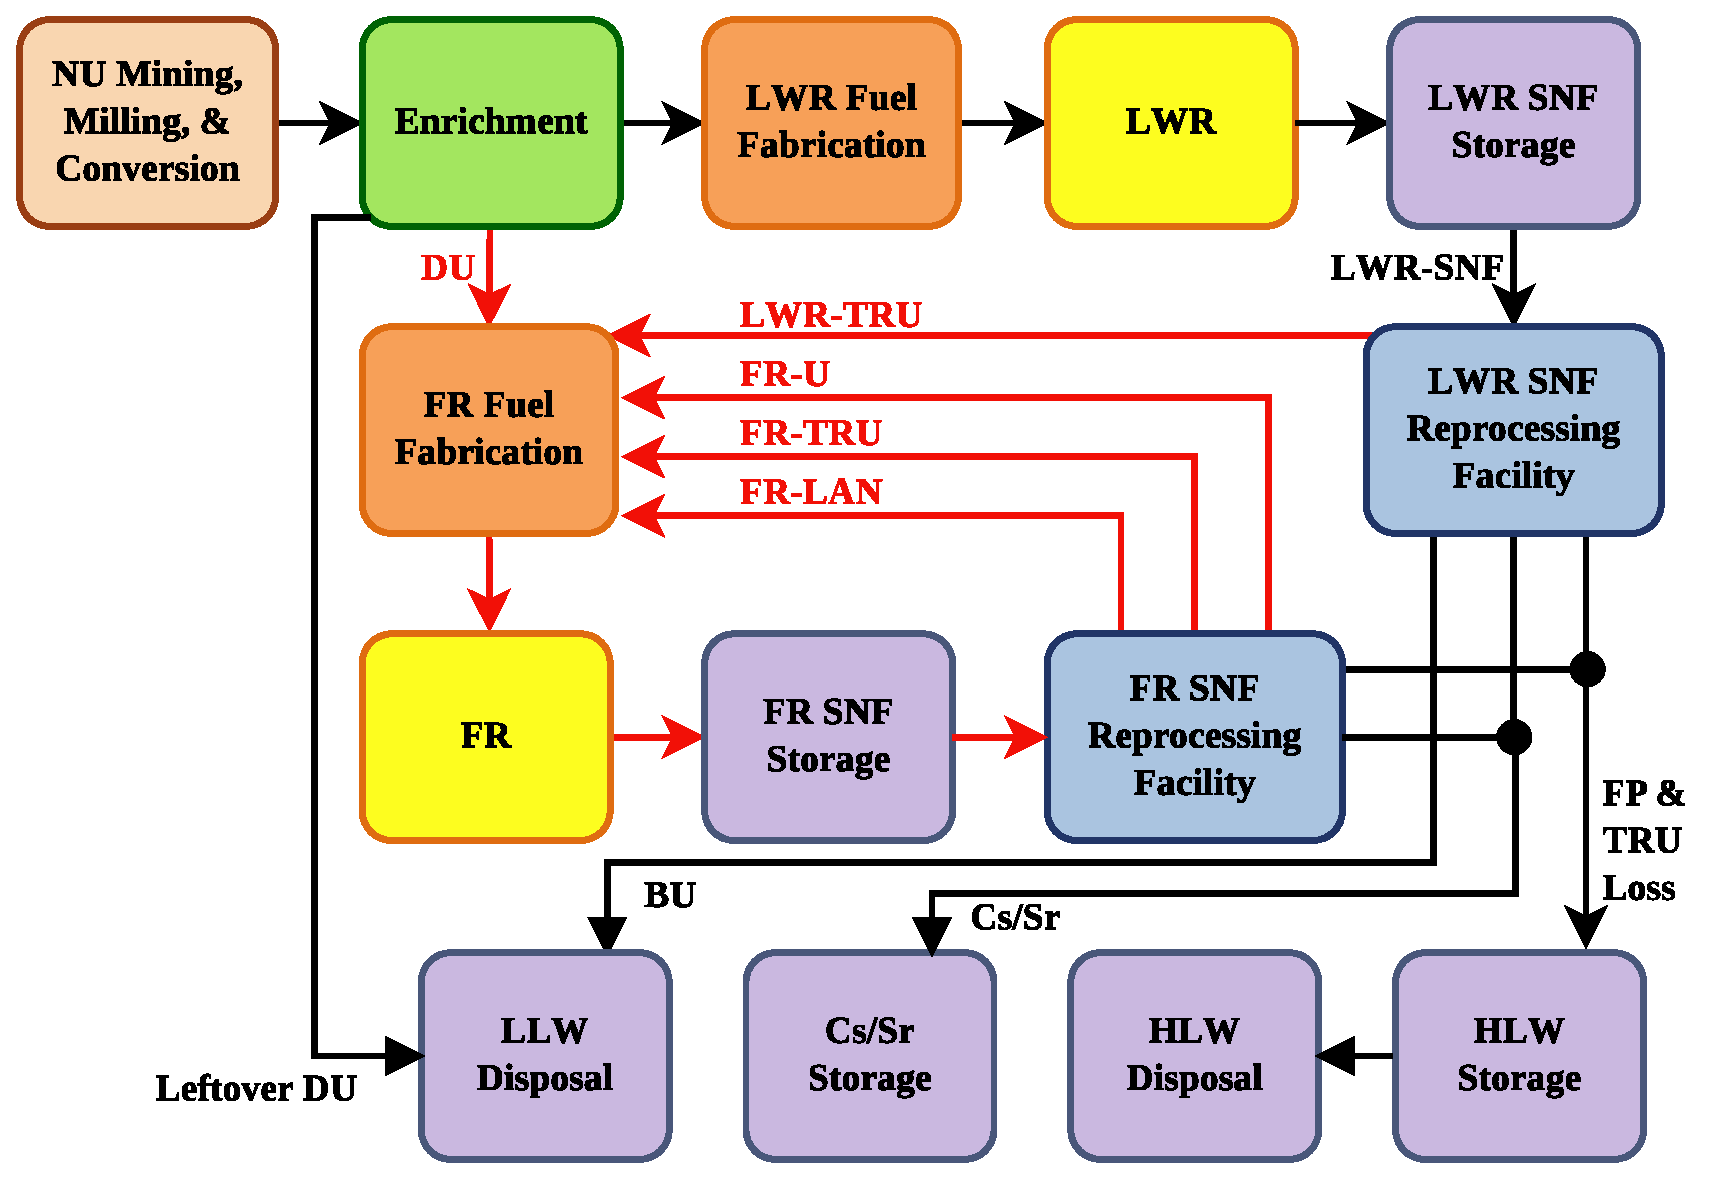
\includegraphics[scale=0.35]{figs/LWR_FR.eps}
\FigCaption{Figure 6: FR-LWR Cycle}
\end{center}
\end{slide}




%Fuel Cycle Benchmark
\overlays{3}{
\begin{slide}{Fuel Cycle Benchmark}
\FromSlide{1}
\begin{itemize}
    \item An LWR benchmark has already been presented.  
        More LWR and FR examples may be found on the website.

\FromSlide{2}
    \item For benchmarks of repository performance, see [3].

\FromSlide{3}
    \item However, since the fuel cycle we are modeling is based off of
        the NEA/OECD Scheme 3a, we performed an integral comparison to the OECD's own results [4].

\FromSlide{1}
\end{itemize}

\FromSlide{3}
\tiny
\textcolor{gray}{\underline{3:} Li, J., Nicholson, M., Proctor,W.C., Yim, M.-S., McNelis, D.N., 2007. 
``\textit{Examining repository loading options to expand yucca mountain repository capacity.}'' 
In: Proc. Advanced Nuclear Fuel Cycles and Systems, GLOBAL, Boise, ID, September.}

\textcolor{gray}{\underline{4:} Nuclear Energy Agency, ``\textit{Advanced Nuclear Fuel 
Cycles and Radioactive Waste Management,}'' - NEA-5990. 2006:1-248.}
\end{slide}}


%Fuel Cycle Benchmark
\begin{slide}{Fuel Cycle Benchmark}
\tiny
\begin{center}
\FigCaption{Table 1: NEA Scheme 3a Benchmark}
\begin{tabular}{|l||c||c|c||c|c|}
\hline
\textbf{Scheme 3a}     & \textbf{NEA} & \textbf{Model\superscript{1}} & \textbf{\% Diff} & \textbf{Model\superscript{2}} & \textbf{\% Diff} \\
\hline
Electricity Share: LWR & 0.632       & 0.619459             & -2.0244 & 0.634907             & +0.4579 \\
\hline
Electricity Share: FR  & 0.368       & 0.380541             & +3.2955 & 0.365093             & -0.7962 \\
\hline
FR SNF: U              & 0.698       & 0.713806             & +2.2143 & 0.715224             & +2.4082 \\
\hline
FR SNF: NP             & 0.0065      & 0.00661961           & +1.8070 & 0.00685174           & +5.1335 \\
\hline
FR SNF: PU             & 0.266       & 0.248059             & -7.2327 & 0.248319             & -7.1204 \\
\hline
FR SNF: AM             & 0.02        & 0.0226796            & 11.8152 & 0.0217317            & +7.9687 \\
\hline
FR SNF: CM             & 0.0098      & 0.00883517           & -10.920 & 0.00787319           & -24.4730\\
\hline
HLW: U                 & 0.013324    & 0.0132681            & -0.4213 & 0.0134448            & +0.8984 \\
\hline
HLW: NP                & 2.26542E-05 & 2.4079E-05           & +5.9173 & 2.41083E-05          & +6.0316 \\
\hline
HLW: PU                & 0.000704797 & 0.000658893          & -6.9668 & 0.000632361          & -11.4548\\
\hline
HLW: AM                & 5.03426E-05 & 5.63068E-05          & 10.5923 & 5.12344E-05          & +1.7405 \\
\hline
HLW: CM                & 2.18151E-05 & 1.99031E-05          & -9.6068 & 1.67094E-05          & -30.5563\\
\hline
HLW: FP                & 0.985876    & 0.985973             & +0.0098 & 0.985831             & -0.0046 \\
\hline
\end{tabular}
\end{center}

1: Model with initial LWR \nuc{U}{235} enrichment of 4.2 w/o. 

2: Model with LWR discharge burnup of 50 MWd/kg.
\end{slide}



%Demo
\overlays{3}{
\begin{slide}{Demo}
\FromSlide{1}
The point of moving to a Bright-like code is that it is fast.

\FromSlide{2}
\vspace{2cm}
Let's look a demonstration for simple a Once-Through cycle where we vary the 
uranium enrichment and observe the maximum discharge burnup.

\FromSlide{3}
\vspace{2cm}
\raggedleft{::cross your fingers::}

\FromSlide{1}
\end{slide}}


%Fuel Cycle Option Space
\overlays{5}{
\begin{slide}{Fuel Cycle Option Space}
\FromSlide{1}
\begin{itemize}
    \item Now that we have a rapid, physics-based fuel cycle model, the 
        types of studies that we may perform increases dramatically. 

\FromSlide{2}
    \item  Unlike other fuel cycle simulators, we can now comprehensively 
        and simultaneously vary many input parameters at once.

\FromSlide{3}
    \item In previous incarnations, we have focused on 1D sensitivity 
        studies for the LWR-FR scenario.  

\FromSlide{4}
    \item Here we are going to examine the same scenario using 
        contingency table analysis.  

\FromSlide{5}
    \item But first, a word from our sophists...

\FromSlide{1}
\end{itemize}
\end{slide}}


%Fuel Cycle Motivation
\overlays{5}{
\begin{slide}{Fuel Cycle Motivation}
\FromSlide{1}
\begin{itemize}
    \item Many nuclear fuel cycle simulations are formulated on premade base-case scenarios:

\FromSlide{2}
    \begin{center}
    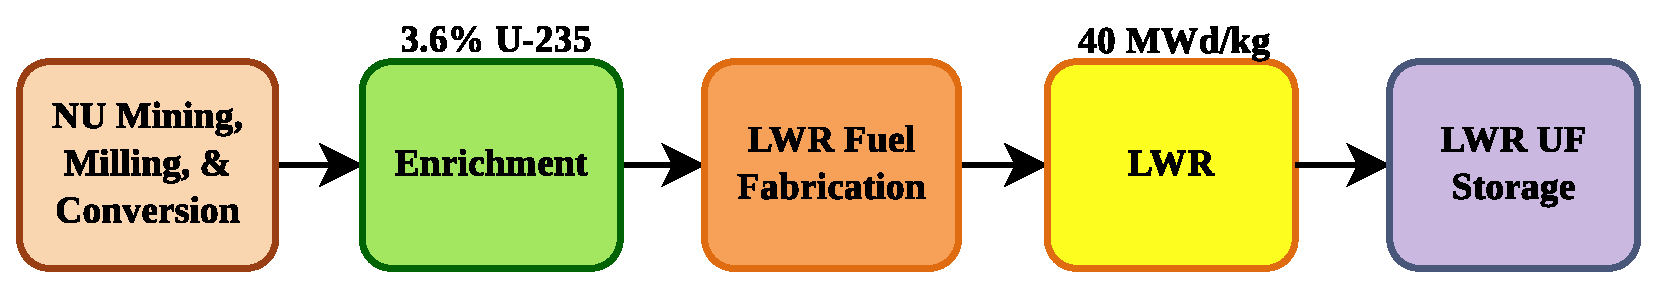
\includegraphics[scale=0.25]{figs/OnceThrough.eps}
    \end{center}

\FromSlide{3}
    \item These base cases are very well studied.

\FromSlide{4}
    \item However, what is \textbf{\textit{not}} well known is 
        how these sample scenarios are affected by perturbations to their 
        initial physical parameters.
            
\FromSlide{1}
\end{itemize}

\FromSlide{5}
\begin{center}
``\textit{Do our parameter choices really give us the `best' solution?}''
\end{center}

\end{slide}}



%Fuel Cycle Methodology
\overlays{4}{
\begin{slide}{Fuel Cycle Methodology}
\FromSlide{1}
\begin{itemize}
    \item Here, we quantify the system-wide impact of physical parameter perturbations.

\FromSlide{2}
    \item This is done by performing \textbf{Contingency Table} analysis for each parameter
        to the \underline{repository} \underline{capacity} response, measured in units of energy.  

\FromSlide{3}
    \item Denote fuel cycle responses as $R$ [GWh] for $x$ input parameters.

\FromSlide{4}
    \item \textbf{\underline{Goal:}} Determine strength of association 
        between inputs and pairs of inputs to the response in a manner that is independent to:
        \begin{itemize}
            \item the functional form of the response to the input $R(x)$,
            \item any base-case set of initial inputs.
        \end{itemize}

\FromSlide{1}
\end{itemize}
\end{slide}}



%Fuel Cycle Methodology
\overlays{3}{
\begin{slide}{Fuel Cycle Methodology}
\FromSlide{1}
\begin{itemize}
    \item In our model, we may adjust over 30 independent physical 
        parameters in the fuel cycle.
\end{itemize}

\FromSlide{2}
\begin{center}
\includegraphics[scale=0.20]{figs/LWR_FR_knobs.eps}
\FigCaption{Figure 2: FR-LWR Cycle with Parameter Representation}
\end{center}

\FromSlide{3}
\begin{itemize}
    \item We present equilibrium results derived from a full treatment
        of the preceding, transient cycles.
\end{itemize}
\end{slide}}




%Input Variable Definition
\begin{slide}{Input Variable Definition}
\tiny
\begin{center}
\begin{tabular}{|l||c|c|c|c|}
\hline
\textbf{Input Parameter $x$} & \textbf{Min} & \textbf{Max} & \textbf{Units} & \textbf{Sample Type}\\
\hline
LWR Burnup Level & 30.0 & 80.0 & MWd/kgIHM & linear \\
\hline
LWR Fuel to Moderator Ratio & 0.28 & 0.36 & & linear \\
\hline
LWR SNF Storage Time & 3 & 30 & years & linear \\
\hline
SE of U from LWR SNF & 0.99 & 0.9999 & & nines \\
\hline
SE of NP from LWR SNF & 0.9 & 0.9999 & & nines \\
\hline
SE of PU from LWR SNF & 0.9 & 0.9999 & & nines \\
\hline
SE of AM from LWR SNF & 0.9 & 0.9999 & & nines \\
\hline
SE of CM from LWR SNF & 0.9 & 0.9999 & & nines \\
\hline
SE of CS from LWR SNF & 0.9 & 0.9999 & & nines \\
\hline
SE of SR from LWR SNF & 0.9 & 0.9999 & & nines \\
\hline
FR Burnup Level & 100.0 & 200.0 & MWd/kgIHM & linear\\
\hline
FR TRU Conversion Ratio & 0.25 & 0.95 & & linear \\
\hline
Max Fraction of Lanthanide in FR Fuel & 0.0001 & 0.005 & Atoms/TRU Atom & linear \\
\hline
FR SNF Storage Time & 3 & 30 & years & linear \\
\hline
Storage Before Disposal & 1 & 300 & years & log \\
\hline
\end{tabular}
\end{center}
\end{slide}

%Input Variable Definition
\begin{slide}{Input Variable Definition}
\tiny
\begin{center}
\begin{tabular}{|l||c|c|c|c|}
\hline
\textbf{Input Parameter $x$} & \textbf{Min} & \textbf{Max} & \textbf{Units} & \textbf{Sample Type}\\
\hline
SE of U from FR SNF & 0.99 & 0.9999 & & nines \\
\hline
SE of NP from FR SNF & 0.9 & 0.9999 & & nines \\
\hline
SE of PU from FR SNF & 0.9 & 0.9999 & & nines \\
\hline
SE of AM from FR SNF & 0.9 & 0.9999 & & nines \\
\hline
SE of CM from FR SNF & 0.9 & 0.9999 & & nines \\
\hline
SE of CS from FR SNF & 0.9 & 0.9999 & & nines \\
\hline
SE of SR from FR SNF & 0.9 & 0.9999 & & nines \\
\hline
Density of Host Rock & 2317 & 2869 & kg/m\superscript{3} & linear \\
\hline
Specific Heat of Host Rock & 590 & 1270 & J/kg-K & linear \\
\hline
Thermal Conductivity of Host Rock & 1.9204 & 3.2856 & W/m-K & linear \\
\hline
Heat Loss Factor During Ventilation  & 0.806 & 0.914 & & linear \\
\hline
Drift diameter & 4.5 & 6.5 & m & linear \\
\hline
Ventilation System On Time & 10 & 300 & years & log \\
\hline
Ambient Environment Temperature & 12.82 & 32.82 & C & linear \\
\hline
Distance Between Drifts & 56 & 106 & m & linear \\
\hline
\end{tabular}
\end{center}
\end{slide}






%Analysis Methodology
\overlays{5}{
\begin{slide}{Analysis Methodology}
\FromSlide{1}
\begin{itemize}
    \item Before attempting to comprehend the subtleties of a 30+ dimensional surface,  
        prudence demands that we check and see if we really need all 30 variables...

\FromSlide{2}
    \begin{itemize}
        \item (Hint: we probably don't!)
    \end{itemize}

\FromSlide{3}
    \item Thus we are looking for a quantitative ranking of the \emph{associations} of each input parameter to the response.  

\FromSlide{4}
    \begin{itemize}
        \item (Note that these associations do not imply a linear response!)
    \end{itemize}

\FromSlide{5}
    \item To do this, we are going to borrow an analysis tool that is often used in Biology: \underline{Contingency Tables}.

\FromSlide{1}
\end{itemize}
\end{slide}}



%Contingency Tables
\overlays{3}{
\begin{slide}{Contingency Tables}
\FromSlide{1}
The $2\times 2$ table is most common:
\begin{center}
\FigCaption{Table 2: Hair Color to Sex Contingency Table}
\begin{tabular}{|l||c|c||c|}
\hline
       & Blonde & Brunette & Totals \\
\hline
Female & 18     & 17       & 35 \\
\hline
Male   & 11     & 14       & 25 \\
\hline
Totals & 29     & 31       & 60 \\
\hline
\end{tabular}
\end{center} 

\FromSlide{2}
\vspace{1.0cm}
But doesn't this approach ignore the underlying biology?

\FromSlide{3}
\vspace{1.0cm}
\raggedleft{\LARGE \textit{Yes!}}
\end{slide}}



%Contingency Tables
\overlays{6}{
\begin{slide}{Contingency Tables}
\begin{center}
\onlySlide*{1}{
\includegraphics[scale=0.125]{figs/CTBlackBox/CTBlackBox01.eps}}

\onlySlide*{2}{\includegraphics[scale=0.125]{figs/CTBlackBox/CTBlackBox02.eps}}

\onlySlide*{3}{
\includegraphics[scale=0.125]{figs/CTBlackBox/CTBlackBox03.eps}}

\onlySlide*{4}{\includegraphics[scale=0.125]{figs/CTBlackBox/CTBlackBox04.eps}}

\onlySlide*{5}{\includegraphics[scale=0.125]{figs/CTBlackBox/CTBlackBox05.eps}}

\onlySlide*{6}{\includegraphics[scale=0.125]{figs/CTBlackBox/CTBlackBox06.eps}}
\end{center}
\end{slide}}



%Fuel Cycle Contingency Table
\overlays{2}{
\begin{slide}{Fuel Cycle Contingency Table}
\FromSlide{1}
For example, let's construct a 2D contingency table that 
measures the response from a sample input: fast reactor 
fuel plutonium separation efficiency, \texttt{FR\_SE\_PU}.

\FromSlide{2}
\vspace{1.0cm}
\tiny
\begin{table}
\caption{Contingency Table for FR Plutonium SE to Repository Capacity [MTHM/Repository].}
\begin{center}
\tiny
\begin{tabular}{|c||c|c|c||c|}
\hline
&$0.9<$\texttt{SE}$<0.99$&$0.99<$\texttt{SE}$<0.999$&$0.999<$\texttt{SE}$<0.9999$&\\
\hline
$10^4 <$ \texttt{Capacity} $< 10^5$&$739$&$43$&$27$&$809$\\
\hline
$10^5 <$ \texttt{Capacity} $< 10^6$&$31510$&$21611$&$19469$&$72590$\\
\hline
$10^6 <$ \texttt{Capacity} $< 10^7$&$2648$&$13095$&$14430$&$30173$\\
\hline
$10^7 <$ \texttt{Capacity} $< 10^8$&$0$&$213$&$1053$&$1266$\\
\hline
&$34897$&$34962$&$34979$&$104838$\\
\hline
\end{tabular}
\end{center}
\label{ct2d_example}
\end{table}

\end{slide}}


%Contingency Table Statistics
\overlays{3}{
\begin{slide}{Contingency Table Statistics}
\FromSlide{1}
There are several metrics that have been developed to measure 
associations with contingency tables.  

\FromSlide{2}
\vspace{0.5cm}
The measure we will be using is the \emph{Uncertainty Coefficient} $U(x|R)$.

\FromSlide{3}
\vspace{0.5cm}
To calculate $U(x|R)$ we will need, 
\begin{itemize}
    \item The \emph{Entropy} $H(x)$, which is a measure of how evenly the 
        data is spread out in the $x$ parameter.
    \item The \emph{Mutual Information} $I(R,x)$ which states the shared
        value of the $x$ together with $R$. 
\end{itemize}
\end{slide}}


%Contingency Table Statistics
\overlays{3}{
\begin{slide}{Contingency Table Statistics}
\FromSlide{1}
Denote the entries in a contingency table as $N_{ij}$ for the i\superscript{th} response bin
and the j\superscript{th} input bin.

\FromSlide{2}
\vspace{0.5cm}
The probability of landing in a given bin is therefore, 
\[ p_{ij} = \frac{N_{ij}}{N} \] 

\FromSlide{3}
\vspace{0.5cm}
We may then calculate the entropy from, 
\[ H(x) = - \sum_j^J p_{\cdot j} \ln(p_{\cdot j}) \]
\end{slide}}


%Contingency Table Statistics
\overlays{2}{
\begin{slide}{Contingency Table Statistics}
\FromSlide{1}
The mutual information is found via, 
\[ I(R,x) = - \sum_{i,j}^{I,J} p_{ij} \ln\left(\frac{p_{ij}}{p_{i\cdot}\cdot p_{\cdot j}}\right) \]

\FromSlide{2}
\vspace{0.5cm}
The relations may be seen graphically:

\vspace{0.5cm}
\setlength{\unitlength}{1cm}
\begin{center}
\begin{picture}(9,3)(-4.5,-1.5)
\thicklines
\put(0,1.5){\vector(1,0){4.5}}
\put(0,1.5){\vector(-1,0){4.5}}
\put(-0.7,1.2){\tiny $H(x,R)$}

\put(-2.25,1.0){\vector(1,0){2.25}}
\put(-2.25,1.0){\vector(-1,0){2.25}}
\put(-2.6,0.7){\tiny $H(x)$}

\put(1.5,0.5){\vector(1,0){3}}
\put(1.5,0.5){\vector(-1,0){3}}
\put(1.2,0.2){\tiny $H(R)$}

\put(-0.75,0){\vector(1,0){0.75}}
\put(-0.75,0){\vector(-1,0){0.75}}
\put(-1.2,-0.3){\tiny $I(R,x)$}

\put(-3,-0.5){\vector(1,0){1.5}}
\put(-3,-0.5){\vector(-1,0){1.5}}
\put(-3.5,-0.8){\tiny $H(x|R)$}

\put(2.25,-0.5){\vector(1,0){2.25}}
\put(2.25,-0.5){\vector(-1,0){2.25}}
\put(2.0,-0.8){\tiny $H(R|x)$}

\end{picture}
\end{center}

\end{slide}}


%Contingency Table Statistics
\overlays{2}{
\begin{slide}{Contingency Table Statistics}
\FromSlide{1}
The uncertainty coefficient is then calculated from,
\[ U(x|R) = \frac{I(R,x)}{H(x)} \]

\FromSlide{2}
This metric has the following useful properties:
\begin{enumerate}
    \item Defined on the range $0 \to 1$.
    \item $U(x|R) = 0$ implies that $I(R,x) = 0$ which indicates that the parameter
        is unassociated with the response.
    \item $U(x|R) = 1$ means that $I(R,x) = H(R) = H(x)$.  This means
        the system response $R(x)$ is solely determined by $x$.
\end{enumerate}
\end{slide}}



%Contingency Table Statistics
\overlays{2}{
\begin{slide}{Contingency Table Statistics}
\FromSlide{1}
\vspace{1cm}
\begin{minipage}[t]{5.0cm}
\begin{center}
\includegraphics[scale=0.25]{figs/Total_Electricity_2D_U_x_R.eps}
\FigCaption{Fig 3: $U(x|R)$ Histogram for Repository Capacity}
\end{center}
\end{minipage}
\FromSlide{2}
\begin{minipage}[t]{5cm}
\tiny
\input{figs/TopBin2D}
\end{minipage}
\end{slide}}



%Conclusions
\overlays{4}{
\begin{slide}{Conclusions}
\FromSlide{1}
\begin{itemize}
    \item We have demonstrated a quick fuel cycle methodology that passes 
        both unit and integral tests.

\FromSlide{2}
    \item Using this new tool, we have developed a robust alternative to simple fuel cycle 
        sensitivity studies using contingency tables and their related statistics.

\FromSlide{3}
    \item This methodology is both quantitative and independent of the functional form 
        between the input and response. 

\FromSlide{4}
    \item In fact, these new metrics do not even require that the stochastic variables 
        be sampled in the same way.


\FromSlide{1}
\end{itemize}
\end{slide}}


%Future Work
\overlays{4}{
\begin{slide}{Future Work}
\FromSlide{1}
\begin{itemize}
    \item On the NFC component side, extending the current reactor methodology from 
        one group to multi-group is an ongoing project.

\FromSlide{2}
    \item Additionally, incorporating a fuel fabrication facility and a repository model 
        into Bright are also ahead.

\FromSlide{3}
    \item Writing Bright bindings for a code like GENIUSv2 would allow us to get the 
        best of both worlds with respect to system-dynamics and physics.

\FromSlide{4}
    \item On the fuel cycle side, applying the contingency table methodology to more system 
        responses and other statistical metrics and increasing table dimensionality will 
        also be done.

\FromSlide{1}
\end{itemize}
\end{slide}}








% Questions
\begin{slide}{Questions}
? ? ? ? ? ? ? ? ? ? ? ? ? ? ? ? ? ? ? ? ? ? ? ? ? ? ? ? ? ? ? 
? ? ? ? ? ? ? ? ? ? ? ? ? ? ? ? ? ? ? ? ? ? ? ? ? ? ? ? ? ? ? 
? ? ? ? ? ? ? ? ? ? ? ? ? ? ? ? ? ? ? ? ? ? ? ? ? ? ? ? ? ? ? 
? ? ? ? ? ? ? ? ? ? ? ? ? ? ? ? ? ? ? ? ? ? ? ? ? ? ? ? ? ? ? 
? ? ? ? ? ? ? ? ? ? ? ? ? ? ? ? ? ? ? ? ? ? ? ? ? ? ? ? ? ? ? 
? ? ? ? ? ? ? ? ? ? ? ? ? ? ? ? ? ? ? ? ? ? ? ? ? ? ? ? ? ? ? 
? ? ? ? ? ? ? ? ? ? ? ? ? ? ? ? ? ? ? ? ? ? ? ? ? ? ? ? ? ? ? 
? ? ? ? ? ? ? ? ? ? ? ? ? ? ? ? ? ? ? ? ? ? ? ? ? ? ? ? ? ? ? 
? ? ? ? ? ? ? ? ? ? ? ? ? ? ? ? ? ? ? ? ? ? ? ? ? ? ? ? ? ? ? 
? ? ? ? ? ? ? ? ? ? ? ? ? ? ? ? ? ? ? ? ? ? ? ? ? ? ? ? ? ? ? 
? ? ? ? ? ? ? ? ? ? ? ? ? ? ? ? ? ? ? ? ? ? ? ? ? ? ? ? ? ? ? 
? ? ? ? ? ? ? ? ? ? ? ? ? ? ? ? ? ? ? ? ? ? ? ? ? ? ? ? ? ? ? 
? ? ? ? ? ? ? ? ? ? ? ? ? ? ? ? ? ?
\end{slide}

\begin{slide}{Bibliography}
\tiny
\begin{enumerate}
    \item \fullcite{Scopatz2009}
    \item \fullcite{Takano1994}
    \item \fullcite{NEA-5990}
\end{enumerate}
\end{slide}

\end{document}
